% Component diagram of the haptic interaction teach-and-record software.
% Requires only \usepackage{tikz}; coordinates are in millimetres, y grows downwards.
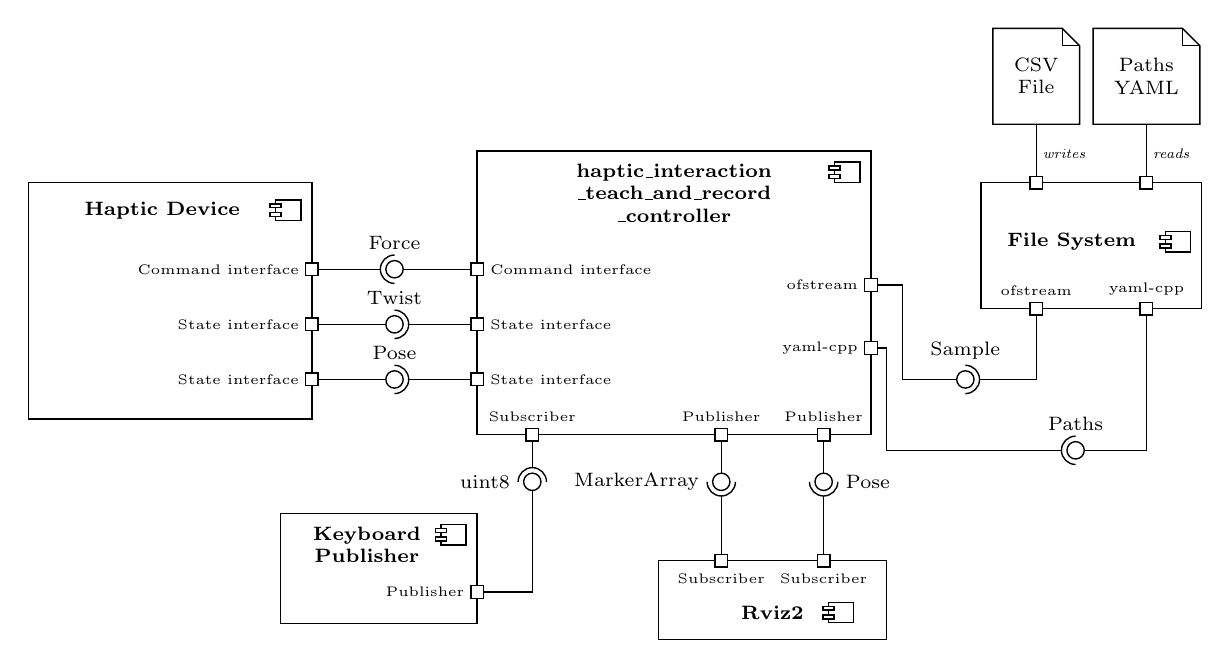
\begin{tikzpicture}[
    x=1mm, y=-1mm,
    line width=0.5pt,
    % Component body
    component/.style={draw, fill=white},
    % Component name
    title/.style={font=\scriptsize\bfseries, align=center, inner sep=0pt},
    % Text next to a port, inside the component
    port label/.style={font=\tiny, inner sep=0.5pt},
    % Name of an interface exchanged between two ports
    iface label/.style={font=\scriptsize, inner sep=1pt},
    % Annotation on a connection
    edge label/.style={font=\tiny\itshape, inner sep=1pt},
    % Note or artifact with a folded top-right corner, sized on its text
    note/.style={
        align=center, font=\scriptsize, inner xsep=2.6mm, inner ysep=1.5mm,
        append after command={
            \pgfextra{
                \draw ([xshift=-2.2mm]\tikzlastnode.north east)
                    -- (\tikzlastnode.north west) -- (\tikzlastnode.south west)
                    -- (\tikzlastnode.south east)
                    -- ([yshift=-2.2mm]\tikzlastnode.north east) -- cycle;
                \draw ([xshift=-2.2mm]\tikzlastnode.north east)
                    |- ([yshift=-2.2mm]\tikzlastnode.north east);
            }
        },
    },
    % File artifact: a note with a fixed minimum size
    artifact/.style={note, minimum width=10mm, minimum height=12mm},
    % Square port centred on a component edge
    pics/port/.style={code={
        \draw[fill=white] (-0.8mm,-0.8mm) rectangle (0.8mm,0.8mm);
    }},
    % UML component icon, anchored at its top-right corner
    pics/component icon/.style={code={
        \draw[fill=white] (-3.2mm,0mm) rectangle (0mm,-2.6mm);
        \draw[fill=white] (-3.9mm,-0.5mm) rectangle (-2.5mm,-1.0mm);
        \draw[fill=white] (-3.9mm,-1.6mm) rectangle (-2.5mm,-2.1mm);
    }},
    % Ball-and-socket assembly connector; the argument is the direction
    % (in degrees, counter-clockwise from the right) the socket faces
    pics/assembly/.style={code={
        \draw ({#1-90}:1.8mm) arc[start angle={#1-90}, end angle={#1+90}, radius=1.8mm];
        \draw[fill=white] (0mm,0mm) circle[radius=1.1mm];
    }},
]

% ---------------------------------------------------------------- Components
% Haptic device
\draw[component] (0,20) rectangle (36,50);
\node[title] at (17,23.5) {Haptic Device};
\pic at (34.6,22.2) {component icon};

% Controller
\draw[component] (57,16) rectangle (107,52);
\node[title, anchor=north] at (82,17.6)
    {haptic\_interaction\\\_teach\_and\_record\\\_controller};
\pic at (105.6,17.4) {component icon};

% File system
\draw[component] (121,20) rectangle (149,36);
\node[title] at (132.5,27.5) {File System};
\pic at (147.6,26.2) {component icon};

% Keyboard publisher
\draw[component] (32,62) rectangle (57,76);
\node[title] at (43,66) {Keyboard\\Publisher};
\pic at (55.6,63.4) {component icon};

% Rviz2
\draw[component] (80,68) rectangle (109,78);
\node[title] at (94.5,74.6) {Rviz2};
\pic at (104.8,73.3) {component icon};

% ---------------------------------------------------------- Notes and files
%\node[note, anchor=east] (sample note) at (116,6.5)
%    {Each sample\\contains position,\\orientation, twist and time.};
\node[artifact] (csv) at (128,6.5) {CSV\\File};
\node[artifact] (yaml) at (142,6.5) {Paths\\YAML};
%\node[note, anchor=north] (path note) at (133,62)
%    {Each path is named\\and contains a\\list of positions.};
%
% ---------------------------------------------------------------- Wiring
% Haptic device <-> controller
\draw (36,31) -- (44.7,31);
\draw (46.5,31) -- (57,31);
\draw (36,38) -- (46.5,38);
\draw (48.3,38) -- (57,38);
\draw (36,45) -- (46.5,45);
\draw (48.3,45) -- (57,45);

% Controller -> file system (recorded samples)
\draw (107,33) -| (111,45) -- (119,45);
\draw (120.8,45) -| (128,36);

% File system -> controller (paths)
\draw (107,41) -| (109,54) -- (131.2,54);
\draw (133,54) -| (142,36);

% Files <-> file system
\draw (csv.south) -- (128,20);
\draw (yaml.south) -- (142,20);

% Keyboard publisher -> controller
\draw (64,52) -- (64,56.2);
\draw (57,72) -| (64,58);

% Controller -> Rviz2
\draw (88,52) -- (88,58);
\draw (88,59.8) -- (88,68);
\draw (101,52) -- (101,58);
\draw (101,59.8) -- (101,68);

% Note attachments
%\draw[dashed] (sample note.east) -- (csv.west);
%\draw[dashed] (133,55.1) -- (path note.north);

% ---------------------------------------------------------------- Ports
\foreach \p in {(36,31), (36,38), (36,45),
                (57,31), (57,38), (57,45), (107,33), (107,41),
                (64,52), (88,52), (101,52),
                (128,20), (142,20), (128,36), (142,36),
                (57,72), (88,68), (101,68)}
    \pic at \p {port};

% Haptic device ports
\node[port label, anchor=east] at (34.6,31) {Command interface};
\node[port label, anchor=east] at (34.6,38) {State interface};
\node[port label, anchor=east] at (34.6,45) {State interface};

% Controller ports
\node[port label, anchor=west] at (58.4,31) {Command interface};
\node[port label, anchor=west] at (58.4,38) {State interface};
\node[port label, anchor=west] at (58.4,45) {State interface};
\node[port label, anchor=east] at (105.6,33) {ofstream};
\node[port label, anchor=east] at (105.6,41) {yaml-cpp};
\node[port label, anchor=south] at (64,50.6) {Subscriber};
\node[port label, anchor=south] at (88,50.6) {Publisher};
\node[port label, anchor=south] at (101,50.6) {Publisher};

% File system ports
\node[port label, anchor=south] at (128,34.6) {ofstream};
\node[port label, anchor=south] at (142,34.6) {yaml-cpp};
\node[edge label, anchor=west] at (128.4,16.3) {writes};
\node[edge label, anchor=west] at (142.4,16.3) {reads};

% Keyboard publisher and Rviz2 ports
\node[port label, anchor=east] at (55.6,72) {Publisher};
\node[port label, anchor=north] at (88,69.4) {Subscriber};
\node[port label, anchor=north] at (101,69.4) {Subscriber};

% ----------------------------------------------------------- Interfaces
\pic at (46.5,31) {assembly=180};
\node[iface label, anchor=south] at (46.5,28.9) {Force};
\pic at (46.5,38) {assembly=0};
\node[iface label, anchor=south] at (46.5,35.9) {Twist};
\pic at (46.5,45) {assembly=0};
\node[iface label, anchor=south] at (46.5,42.9) {Pose};

\pic at (119,45) {assembly=0};
\node[iface label, anchor=south] at (119,42.9) {Sample};
\pic at (133,54) {assembly=180};
\node[iface label, anchor=south] at (133,51.9) {Paths};

\pic at (64,58) {assembly=90};
\node[iface label, anchor=east] at (61.6,58) {uint8};
\pic at (88,58) {assembly=270};
\node[iface label, anchor=east] at (85.6,58) {MarkerArray};
\pic at (101,58) {assembly=270};
\node[iface label, anchor=west] at (103.4,58) {Pose};

\end{tikzpicture}